Global menu jest funkcjonalnością pulpitu Ubuntu Unity polegającą na przeniesieniu paska menu programu (opcje takie jak \menu{Plik} \menu{Edycja} czy \menu{Narzedzia} z okna programu na główną belkę unity (górny pasek menu). Po uruchomieniu dowolnej aplikacji pasek menu zawiera jedynie nazwę aktualnie aktywnego okna:

\begin{center}
	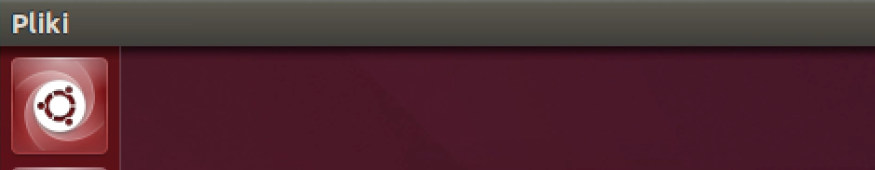
\includegraphics[width=\linewidth]{images/unity_menu_bar2.png}
\end{center}

Pasek manu jest aktywowany, gdy kursor myszy znajdzie się w obrębie panelu menu:

\begin{center}
	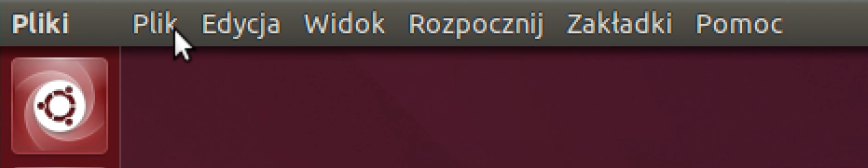
\includegraphics[width=\linewidth]{images/unity_menu_bar3.png}
\end{center}

Jeżeli korzystasz jedynie ze zmaksymalizowanych aplikacji to Global Menu nie przeszkadza. Na ekranach panoramicznych lepiej jest wykorzystywane dostępne miejsce w pionie. Sprawa jednak się komplikuje kiedy korzystamy z okien w ich normalnym rozmiarze z nie zmaksymalizowanych. Aby dostać się do menu trzeba najpierw przesunąć kursor myszy na samą górę ekranu a dopiero potem wybrać odpowiednią opcję. Na szczęście można to zmienić i zintegrować pasek narzędzi programu z jego aktualną belką tytułową. 

Opcja ta jest dostępna poprzez:
\noindent \menu{{Ustawienia systemu}>{Wygląd}>{Zachowanie}>{Pokazuj menu okna}>{W belce tytułowej okna}}